\documentclass[a4paper,10pt,landscape,twocolumn]{scrartcl}

%% Settings
\newcommand\problemset{5}
\newcommand\deadline{Wednesday October 5th, 22:00h}
\newif\ifcomments
\commentsfalse % hide comments
%\commentstrue % show comments

% Packages
\usepackage[english]{exercises}
\usepackage{wasysym,hyperref,graphicx,color}
\hypersetup{colorlinks=true, linkcolor=blue, urlcolor=blue}
\DeclareMathOperator{\Cov}{Cov}
\DeclareMathOperator{\Cor}{Cor}
\DeclareMathOperator{\Var}{Var}

\newcommand{\philip}[1]{\textcolor{red}{[Phil: #1]}}
\newcommand{\chris}[1]{\textcolor{blue}{[Chris: #1]}}

\begin{document}

\homeworkproblems

{\sffamily\noindent
%This week's exercises deal with sets, counting and uniform probabilities.
Your homework must be handed in \textbf{electronically via Moodle before \deadline}.  This deadline is strict and late submissions are graded with a 0. At the end of the course, the lowest of your 7 weekly homework grades will be dropped. You are strongly encouraged to work together on the exercises, including the homework. However, after this discussion phase, you have to write down and submit your own individual solution. Numbers alone are never sufficient, always motivate your answers.
}
%%%%%%%%%%%%%%%%%%%%%%%%%%%%%%%%%%%%%%%%%%%%%%%%%%%

\begin{exercise}[Markov's inequality (2pt)]
	Let $X$ be a random variable and $a > 0$ some real constant. Prove 
	\emph{Markov's Inequality}:
	\[
	P(|X| \ge a) \le \frac{E[|X|]}{a},
	\]
	where $|X|$ is the \href{https://en.wikipedia.org/wiki/Absolute_value}{absolute value} of $X$.
\end{exercise}


\begin{exercise}[Poisson distribution (3pt)]
	The \emph{Poisson distribution} models how often some event happens in a given period of time. Its probability mass function is given by
	\[
	P(X = k) = {\frac {\lambda ^{k}e^{-\lambda }}{k!}}, \qquad \lambda \in \mathbb{R}_{>0}, \quad k=0,1,2,\dots
	\]
	where $\lambda$ is the distribution's only parameter. 
	Let $X_1^N := X_1, \dots, X_N$ be $N$ independent and identically distributed (i.i.d.) random variables following a $\text{Poisson}(\lambda)$ distribution.
		
	\begin{subex}[1pt]
	Let $T(x_1, \dots, x_N) = \sum_{i=1}^N x_i$ be a
        statistic. Show that $T$ is a sufficient statistic for the
        Poisson distribution. \emph{Hint: use the Factorization
          Theorem~5.13 from the script).}
	\end{subex}

	\begin{subex}[0.5pt]
	Find the log-likelihood $\mathcal L_x(\lambda) = \ln P(X_1^N =
        x_1^N\mid \lambda)$ of the data.
	\end{subex}
	
	\begin{subex}[0.5pt]
		Find the derivative $\frac{\partial}{\partial \lambda} \mathcal L(\lambda)$ of the log-likelihood.
	\end{subex}
	
	\begin{subex}[1pt]
		Show that the maximum-likelihood estimate for $\lambda$ is
		\[
			\lambda_\textsc{ml} = \text{argmax}_\lambda
                        P(X_1^N = x_1^N \mid \lambda) = \frac{1}{N}\sum_{i=1}^N x_i.
		\]
	\end{subex}
	
\end{exercise}

%\begin{exercise}[Multiple binomials (2pt)]
%%	\philip{In accordance with our notation, I lowercased all RVs that are arguments to a pmf.}
%	Let $X_1, \dots, X_N$ be i.i.d.\ $\text{Binom}(n, \theta)$ random variables. 
%%	Show that the maximum likelihood estimator for $\lambda$ is:
%%	\[
%%		\theta_\textsc{mle} = \text{argmax}_\lambda P(X_1, \dots, X_N \mid \lambda) = \frac{\sum_{i=1}^N x_i}{n \cdot N}.
%%	\] 
%%	Note that this differs from the script since we now have $N$ rather than 1 random variable. 
%	(Be careful not to confuse $n$ and $N$).
%	
%	\begin{subex}[0.5pt]
%	Find the log-likelihood $\ln P(X_1^N=x_1^N \mid n, \theta)$ of the data.
%	\end{subex}
%	
%	\begin{subex}[0.5pt]
%		Find the derivative $\frac{\partial}{\partial \theta} \ln P(X_1^N=x_1^N \mid n, \theta)$.
%	\end{subex}
%	
%	\begin{subex}[1pt]
%		Show that the maximum likelihood estimator for $\theta$ is (keeping $n$ fixed):
%		\[
%			\theta_\textsc{mle} = \text{argmax}_\theta P(X_1^N=x_1^N \mid n, \theta) = \frac{\sum_{i=1}^N x_i}{n \cdot N}.
%		\] 
%	\end{subex}
%	
%\end{exercise}

\begin{figure}
	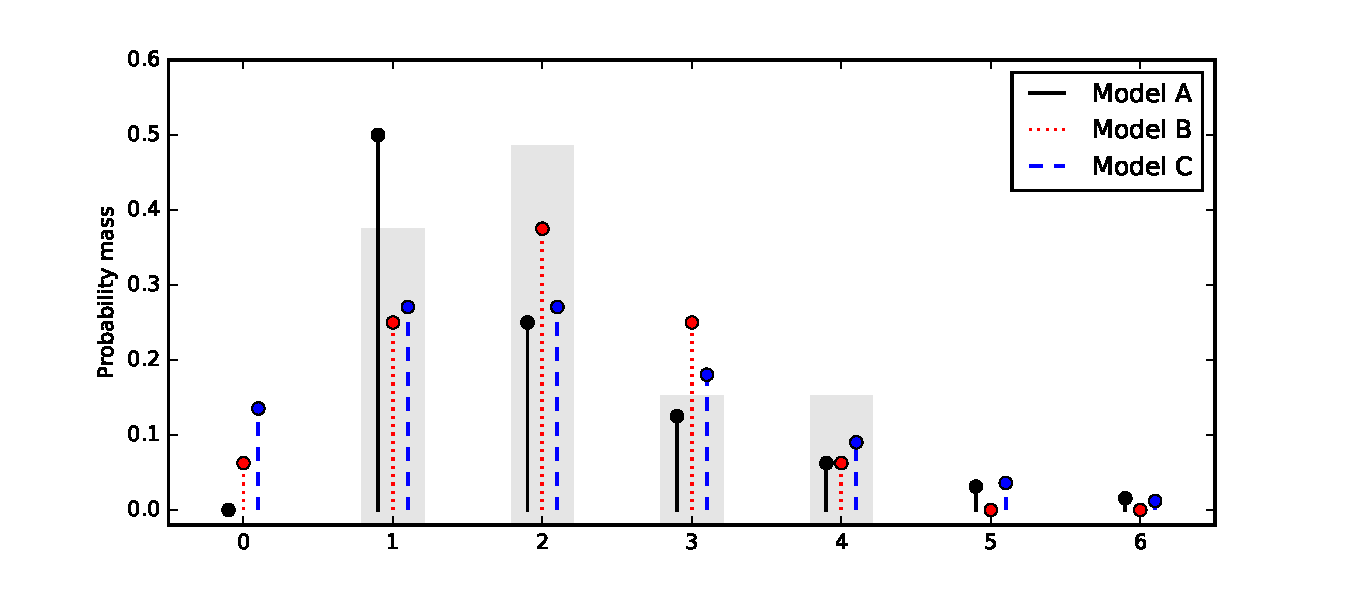
\includegraphics[width=.5\textwidth]{media/05-distributions}
	\caption{Distributions of the three models using the $\textsc{ml}$-parameters. The grey bars in the background show the empirical distribution of the observations, i.e. the relative frequency of all observations in $\mathcal{D}$.\label{fig:models}}
\end{figure}


\begin{exercise}[Three models (3pt)]
Once upon a time, three data enthusiasts, Alice, Bob and Charlie, were asked to look into a dataset that was as small as it was confidential. The client could not provide any information about the dataset, so just gave the data:
	\[
		\mathcal{D} = \{ 1, 1, 2, 4, 2, 1, 3, 2, 2 \}.
	\]
	Puzzled, all three came up with different explanations of the data. Alice thought the data was drawn from a geometric distribution, Bob proposed a binomial distribution and Charlie a Poisson distribution (see Problem~2). More precisely, they assume that the data is generated by $N = |\mathcal D|=9$ i.i.d. random variables, but everyone proposes different ones:
	\begin{align}
		\text{Model Alice:} \quad A_i &\sim \text{Geom}(\pi),\\
		\text{Model Bob:} \quad B_i &\sim \text{Binom}(n, \theta), \quad n=4\\
		\text{Model Charlie:} \quad C_i &\sim \text{Poisson}(\lambda),
	\end{align}
	for $i = 1, \dots, N$. So Alice, Bob and Charlie suppose that the observation $x_1 \in \mathcal D$ is the value taken by the RV $A_1, B_1$ and $C_1$ respectively.
	
	\begin{subex}[0.5pt]
	Bob has already decided on one of the parameters: $n=4$. But all remaining parameters have to be estimated from the data. Calculate the \textsc{ml}-estimates for $\pi$, $\theta$ and $\lambda$ from the data. The distributions of the resulting models are shown in Figure \ref{fig:models}. 
	\emph{Hint: use homework problem 5.2, 5.3 and this week's board questions}.
	\end{subex}
	
	\begin{subex}[0.5pt]
		Calculate the log-likelihood of the data $\mathcal D$ for each of the three models, using the \textsc{ml}-estimates from (a) as parameters. Which model gives the best explanation of the data, i.e. assigns the data the highest likelihood? \emph{Hint: you might find Table \ref{table} useful}.
	\end{subex}
	
	\begin{subex}[1pt]
		Alice, Bob and Charlie wonder how their models differ. Show that all models have the same expectation when parametrised with their respective MLE parameters. Observe that this expectation is equal to the sample mean $\overline x := \frac{1}{N} \sum_{j=1}^N x_j$, where $x_j$ is an observations. However, the models have different variances: show that $\Var(C_i) < \Var(B_i) \le \Var(A_i)$ if $\overline x \ge 2$. 	\end{subex}
	
	\begin{subex}[0.5pt]
		In order to better decide which model is the best, the client provides some more data. The full
		data set now is:
		\[
			\mathcal D' = \mathcal D \cup \{ 0, 4, 5 \}
		\]
		Which model(s) cannot account for this data? In other words, under which model(s) does this data get likelihood 0?
	\end{subex}
	
	\begin{subex}[1pt]
	Let's call the parameter of the one remaining model	$\gamma_\textsc{ml}$. It's inventor actually had a competing hypothesis for the parameter: $\gamma_\textsc{ml}' = 1.25 \times \gamma_\textsc{ml}$, which s/he deemed slightly less likely: $P(\gamma_\textsc{ml}') = 0.4$ while $P(\gamma_\textsc{ml}) = 0.6$. Which of these two parameter should s/he prefer after observing the full data set $\mathcal{D'}$? Answer that question by calculating the posterior $P(\gamma \mid \mathcal{D'})$.
	\end{subex}
	
	\bigbreak\noindent
	\emph{Working with actual data means many computations. That's why you normally want to do this using a computer --- not the human, but the electronic one. You can learn more about that in the follow-up course \emph{Basic Probability: programming}.}
\end{exercise}

\begin{table}
\begin{tabular}{l c c c}
& 	$X \sim \text{Geom}(\pi_\textsc{ml})$
&	$X \sim \text{Binom}(4, \theta_\textsc{ml})$
&	$X \sim \text{Poisson}(\lambda_\textsc{ml})$ \\\hline\hline
$\ln P(X = 0)$ &$-\infty$ &$-2.7726$ &$-2.0000$ \\\hline
$\ln P(X = 1)$ &$-0.6931$ &$-1.3863$ &$-1.3069$ \\\hline
$\ln P(X = 2)$ &$-1.3863$ &$-0.9808$ &$-1.3069$ \\\hline
$\ln P(X = 3)$ &$-2.0794$ &$-1.3863$ &$-1.7123$ \\\hline
$\ln P(X = 4)$ &$-2.7726$ &$-2.7726$ &$-2.4055$ \\\hline
$\ln P(X = 5)$ &$-3.4657$ &$-\infty$ &$-3.3218$ \\\hline
%$\ln P(X = 6)$ &$-4.1589$ &$-\infty$ &$-4.4204$ \\\hline
\end{tabular}
\caption{Some log-probabilities for the three models \label{table}}
\end{table}


\end{document}